\section{ 处理PWM的相关函数 }
\subsection{ PWM初始化函数, 用于初始化PWM配置 }
\begin{figure}[h]
    \centering
    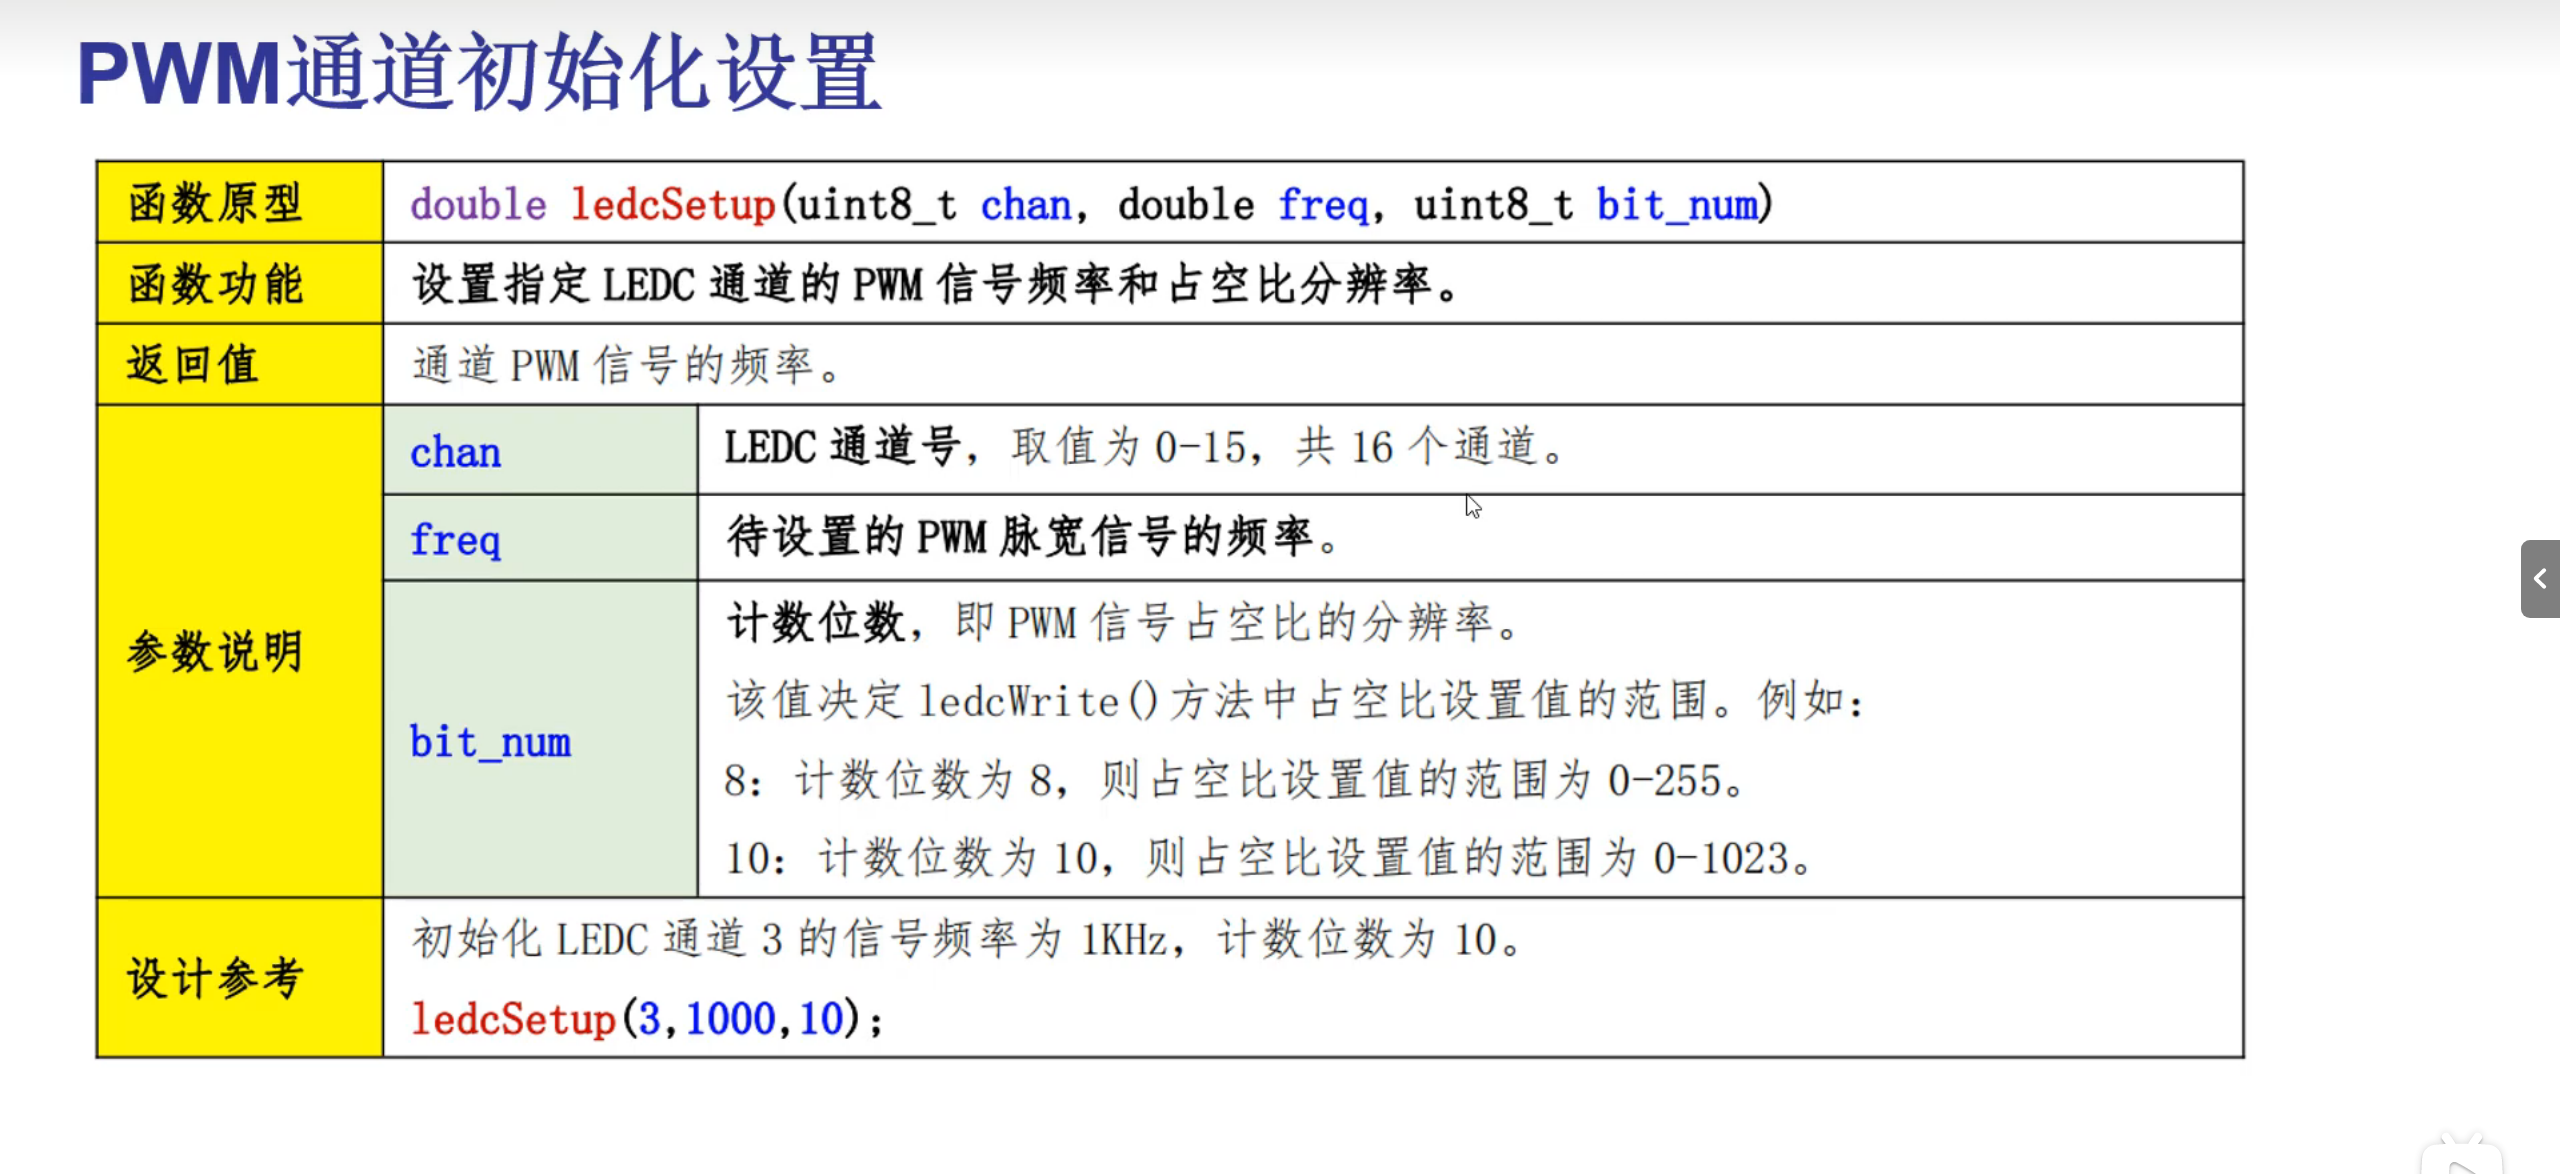
\includegraphics[width=0.6\textwidth]{Figures/ledcSetup.png}
    \caption{ledcSetup}
   
\end{figure}
函数名为:\textit{ \textbf{ void ledcSetup(参数一,参数二,参数三)}  },参数一为要绑定的通道;参数二为PWM频率;参数三为计数位数
\subsection{ PWM通道绑定函数, 用于使能某个特定的引脚输出PWM波 }
\begin{figure}[h]
    \centering
    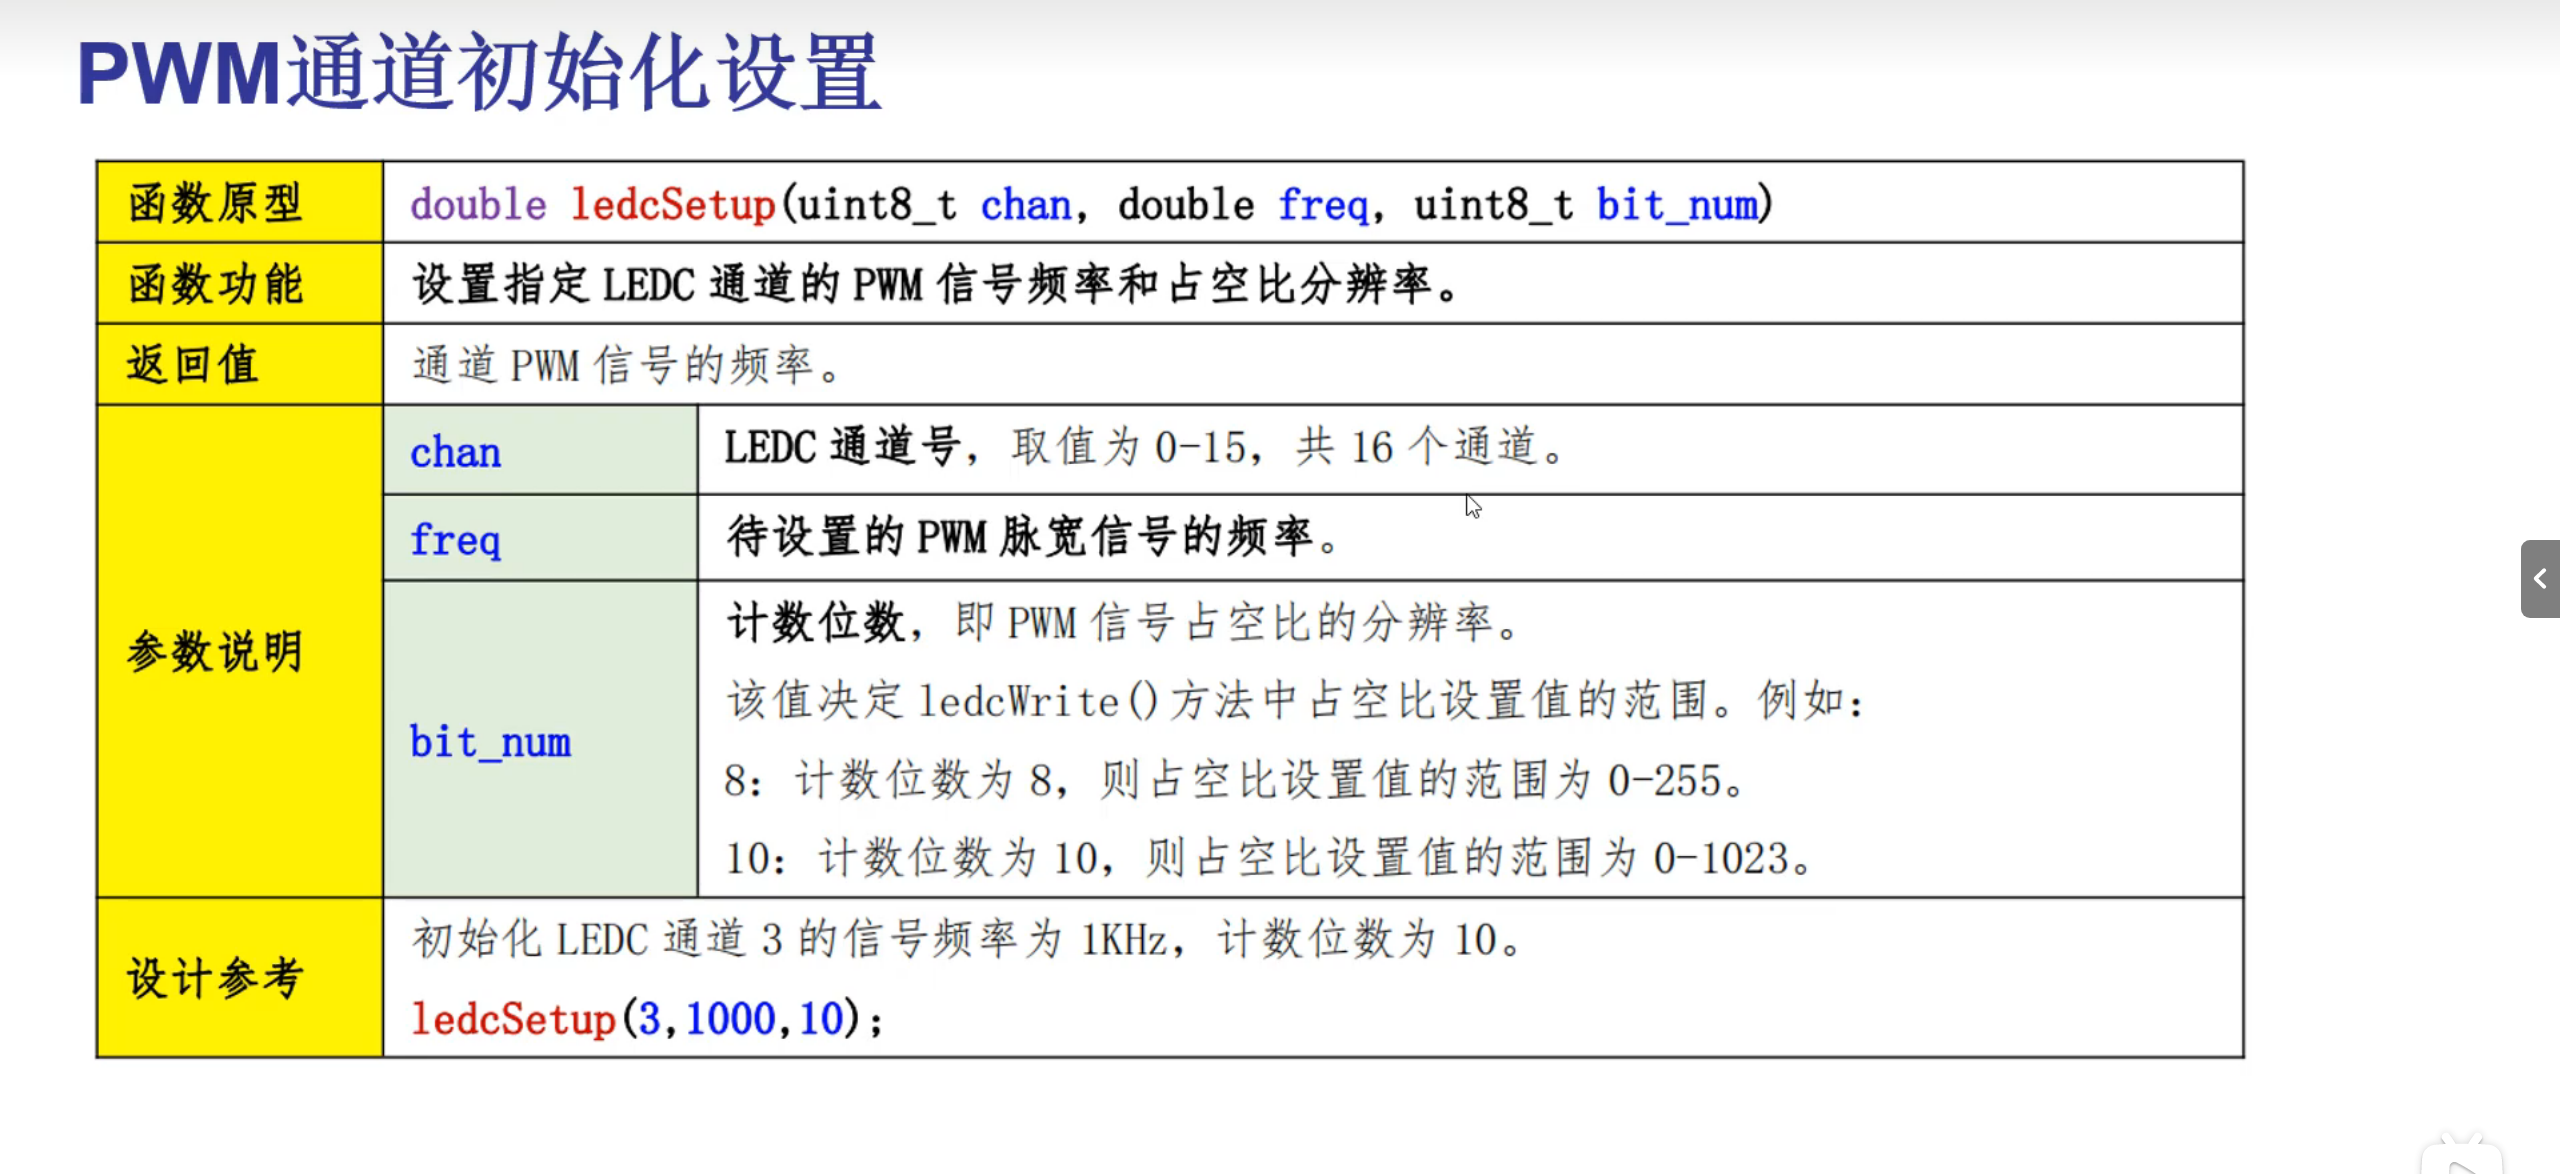
\includegraphics[width=\textwidth]{Figures/ledcAttachPin.png}
    \caption{ledaAttachPin}    
\end{figure}
函数名为:\textit{ \textbf{void ledcAttachPin(参数一,参数二)}}.参数一为要指定的引脚,参数二表示要用哪个通道输出的PWM波

\subsection{ PWM占空比设置函数 }
函数名为: \textit{ \textbf{void ledcWrite(参数一, 参数二 )} }.参数一为要进行操作的PWM通道;参数二为占空比数值
\begin{figure}[h]
    \centering
    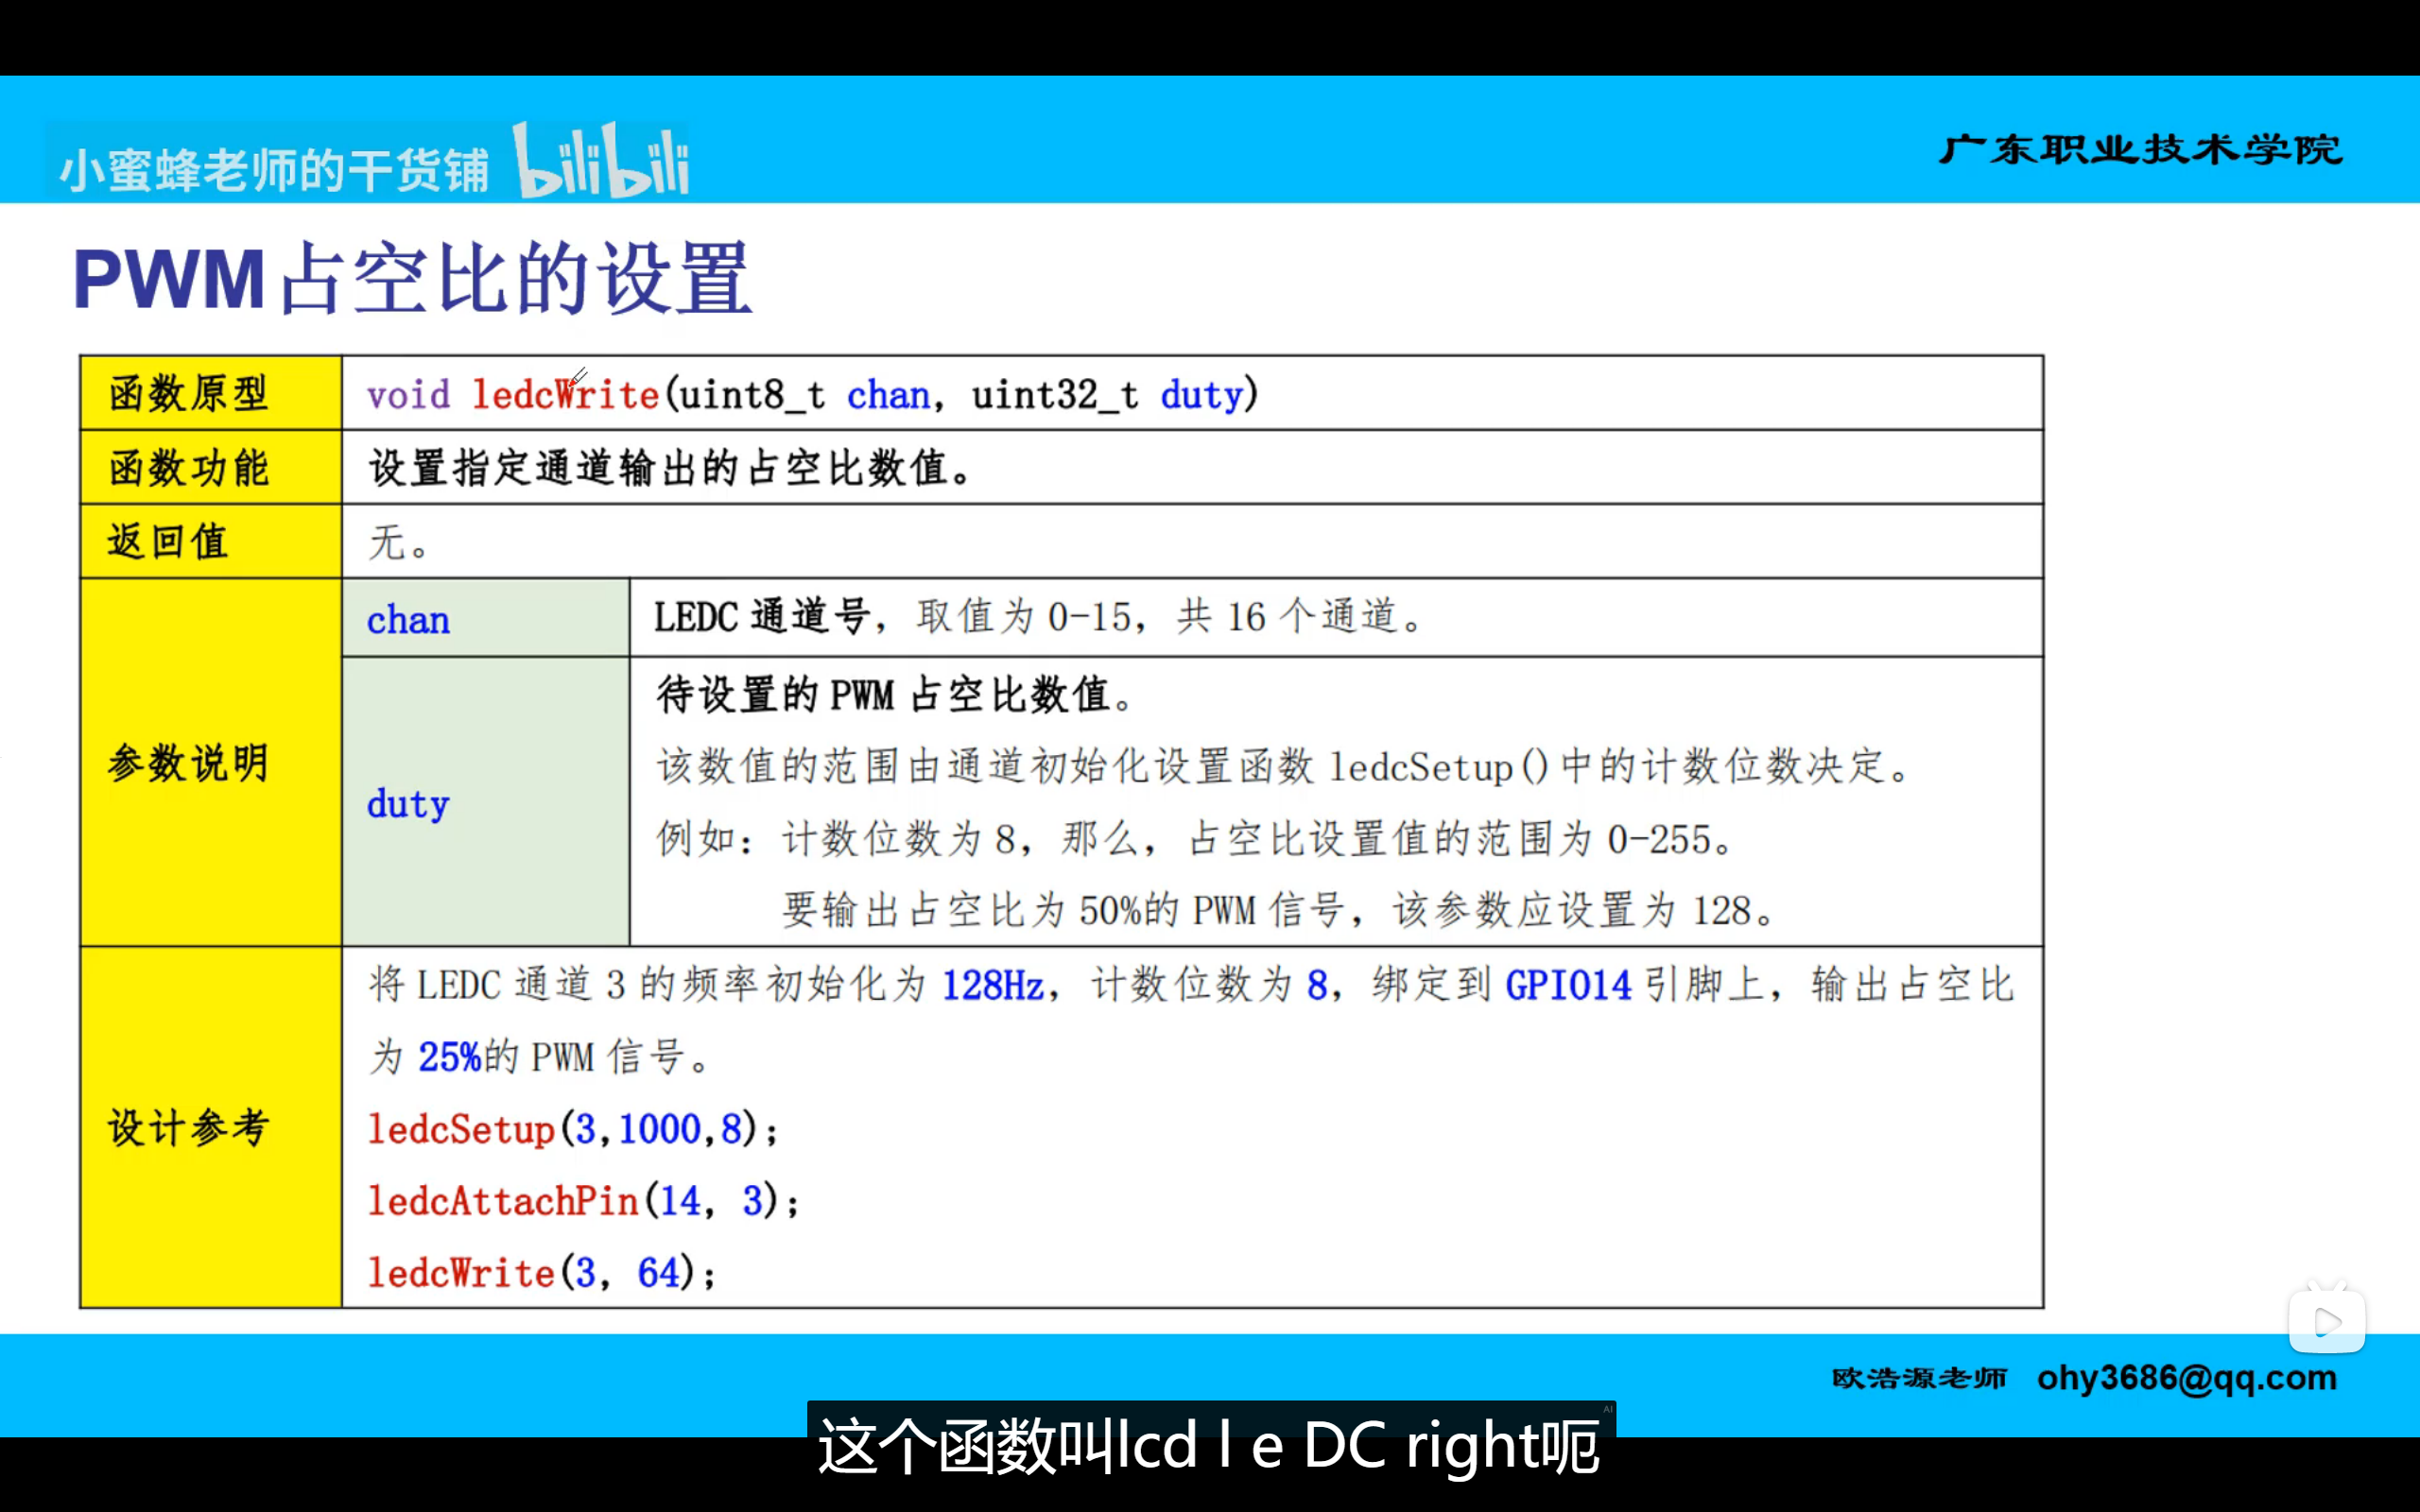
\includegraphics[width=\textwidth]{Figures/ledcWrite.png}
    \caption{ledcWrite}    
\end{figure}